\documentclass{article}

\usepackage[utf8]{inputenc}
\usepackage[T1]{fontenc}
\usepackage[spanish]{babel}
\usepackage{times}
\usepackage{wrapfig}
\usepackage{lmodern}
\usepackage{mathtools}
\usepackage{graphicx}
\usepackage[utf8]{inputenc}
\usepackage{color}
\usepackage{hyperref}
\usepackage{fancyhdr,lipsum}


\hypersetup{
    colorlinks=true, %set true if you want colored links
    linktoc=all,     %set to all if you want both sections and subsections linked
    linkcolor=blue,  %choose some color if you want links to stand out
}

\definecolor{gray97}{gray}{.97}
\definecolor{gray75}{gray}{.75}
\definecolor{gray45}{gray}{.45}

%definir los marcos, fondos, numero y demás de los códigos de SQL
\usepackage{listings} 
  \lstset{ frame=Ltb,
          framerule=0pt,
          aboveskip=0.5cm,
          framextopmargin=3pt,
          framexbottommargin=3pt,
          framexleftmargin=0.4cm,
          framesep=0pt,
          rulesep=.4pt,
          backgroundcolor=\color{gray97},
          rulesepcolor=\color{black},
          %
          stringstyle=\ttfamily,
          showstringspaces = false,
          basicstyle=\small\ttfamily,
          commentstyle=\color{gray45},
          keywordstyle=\bfseries,
          %
          numbers=left,
          numbersep=15pt,
          numberstyle=\tiny,
          numberfirstline = false,
          breaklines=true,
  }

% minimizar fragmentado de listados
\lstnewenvironment{listing}[1][]{\lstset{#1}\pagebreak[0]}{\pagebreak[0]}
\lstdefinestyle{consola}{basicstyle=\scriptsize\bf\ttfamily, backgroundcolor=\color{gray75}, }
\lstdefinestyle{C}{language=C,}

\title{Tarea 3.- Creación de la base de datos \textbf{INMOBILIARIA}}
\author{Antonio Muñoz Cubero}
 

\begin{document}
  \maketitle
    \pagenumbering{gobble}
      \pagestyle{fancy} 

\newpage
  \tableofcontents
    \lhead[BD INMOBILIARIA]{BD INMOBILIARIA}
    \lfoot[IES Francisco De Los Rios]{IES Francisco De Los Rios}
      \pagenumbering{arabic}

\newpage
  \section{Foto del Modelo Relacional}
    \begin{figure}[h]
      \centering
      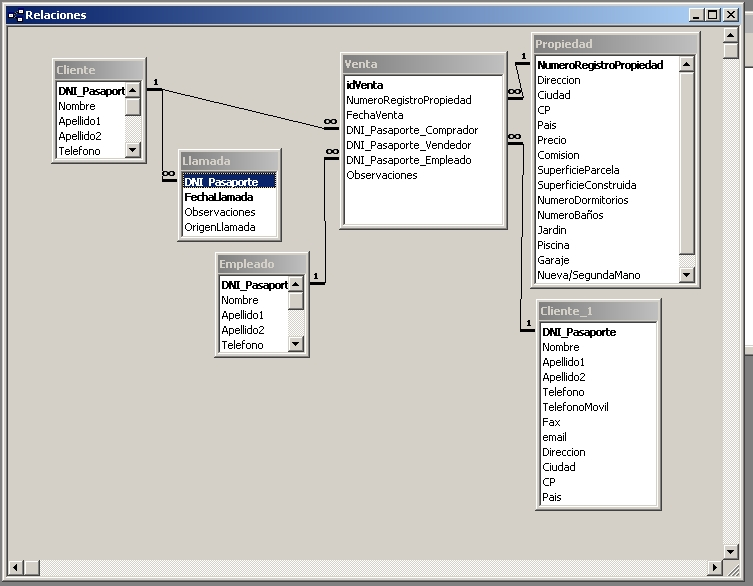
\includegraphics[scale = 0.7]{img/enunciado.png}
      \caption{Foto del Modelo Relacional desde el que partimos.}
    \end{figure}

\newpage
  \section{Creación de la Base de Datos}
    Entramos al cliente de MariaDB con el usuario que tengamos para trabjar, acto seguido empezaremos creando 
    la base de datos \textbf{inmobiliaria} usando los siguientes comandos, después la seleccionamos y comenzamos la creación de las tablas. 
    \begin{listing}[style=consola, numbers=none]
    MariaDB [(none)]> CREATE DATABASE IF NOT EXISTS inmobiliaria;

    MariaDB [(none)]> USE inmobiliaria;

    \end{listing}

  \section{Creación de las tablas}
    \subsection{Tabla 'Comprador'}
      \begin{lstlisting}[style=C]
        CREATE TABLE IF NOT EXISTS Comprador(
          dniComprador INT(10) AUTO_INCREMENT,
          nombre VARCHAR(100) NOT NULL,
          apellido1 VARCHAR(100) NOT NULL,
          apellido2 VARCHAR(100) NOT NULL,
          telefono VARCHAR(9) NOT NULL,
          CONSTRAINT pk_Comprador_dniComprador PRIMARY KEY (dniComprador),
          CONSTRAINT u_Comprador_telefono UNIQUE (telefono)
        )
        ENGINE = InnoDB
        COMMENT ='Tabla donde se almacenan los Compradores que hay en la base de datos'
        ;
      \end{lstlisting}

  \newpage
    \subsection{Tabla 'Empleado'}
      \begin{lstlisting}[style=C]
        CREATE TABLE IF NOT EXISTS Empleado(
          dniEmpleado INT(10) AUTO_INCREMENT,
          nombre VARCHAR(100) NOT NULL,
          apellido1 VARCHAR(100) NOT NULL,
          apellido2 VARCHAR(100) NOT NULL,
          telefono VARCHAR(9) NOT NULL,
          CONSTRAINT pk_Empleado_dniEmpleado PRIMARY KEY (dniEmpleado),
          CONSTRAINT u_Empleado_telefono UNIQUE (telefono)
        )
        ENGINE = InnoDB
        COMMENT ='Tabla donde se almacenan los empleados que hay en la base de datos'
        ;
      \end{lstlisting}

  %\newpage
    \subsection{Tabla 'Llamada'}
      \begin{lstlisting}[style=C]
        CREATE TABLE IF NOT EXISTS Llamada(
          dniComprador INT(10) AUTO_INCREMENT,
          fechaLlamada DATETIME,
          observaciones TEXT DEFAULT 'Ninguna',
          origenLlamada VARCHAR(9) NOT NULL,
          CONSTRAINT pk_Llamada_dniComprador_fechaLlamada PRIMARY KEY (dniComprador,fechaLlamada),
          CONSTRAINT fk_Llamada_dniComprador FOREIGN KEY (dniComprador) REFERENCES Comprador (dniComprador)
        )
        ENGINE = InnoDB
        COMMENT ='Tabla donde se almacenan un registro de llamadas de los Compradores, he considerado que "fechaLlamada" es un DATETIME, 
        ya que al ser pk no puede repetirse y considero que puedes hacer varias llamadas el mismo dia, pero no el mismo dia y a la misma hora.
        Tambien considero que "origenLlamada" almacena un telefono, por eso lo determino como VARCHAR(9)'
        ;
      \end{lstlisting}

  \newpage
    \subsection{Tabla 'Vendedor'}
      \begin{lstlisting}[style=C]
        CREATE TABLE IF NOT EXISTS Vendedor(
          dniVendedor INT(10) AUTO_INCREMENT,
          nombre VARCHAR(100) NOT NULL,
          apellido1 VARCHAR(100) NOT NULL,
          apellido2 VARCHAR(100) NOT NULL,
          telefono VARCHAR(9) NOT NULL,
          telefonoMovil VARCHAR(9) NOT NULL,
          fax VARCHAR(9) NOT NULL,
          email VARCHAR(100) NOT NULL,
          direccion VARCHAR(100) NOT NULL,
          ciudad VARCHAR(100) NOT NULL,
          cp VARCHAR(5) NOT NULL,
          pais VARCHAR(100) NOT NULL,
          CONSTRAINT pk_Vendedor_dniVendedor PRIMARY KEY (dniVendedor),
          CONSTRAINT u_Vendedor_telefono UNIQUE (telefono),
          CONSTRAINT u_Vendedor_telefonoMovil UNIQUE (telefonoMovil),
          CONSTRAINT u_Vendedor_fax UNIQUE (fax),
          CONSTRAINT u_Vendedor_email UNIQUE (email)
        )
        ENGINE = InnoDB
        COMMENT ='Tabla donde se almacenan los vendedores que hay en la base de datos'
        ;
      \end{lstlisting}

    \subsection{Tabla 'Propiedad'}
      \begin{lstlisting}[style=C]
        CREATE TABLE IF NOT EXISTS Propiedad(
          numeroRegistroPropiedad INT(10) AUTO_INCREMENT,
          direccion VARCHAR(100) NOT NULL,
          ciudad VARCHAR(100) NOT NULL,
          cp VARCHAR(5) NOT NULL,
          pais VARCHAR(100) NOT NULL,
          precio INT(20) NOT NULL,
          comision INT(20) NOT NULL,
          superficieParcela INT(40) NOT NULL,
          superficieConstruida INT(40) NOT NULL,
          numeroDormitorios INT(10) NOT NULL,
          numeroBanos INT(10) NOT NULL,
          jardin BOOLEAN NOT NULL,
          piscina BOOLEAN NOT NULL,
          garaje BOOLEAN NOT NULL,
          nuevaSegundaMano BOOLEAN NOT NULL,
          CONSTRAINT pk_Propiedad_numeroRegistroPropiedad PRIMARY KEY (numeroRegistroPropiedad)
        )
        ENGINE = InnoDB
        COMMENT ='Tabla donde se almacenan las propiedades que hay en la base de datos
        en el valor "nuevaSegundaMano" 0 -> nueva | 1-> Segunda mano'
        ;
      \end{lstlisting}

      \subsection{Tabla 'Venta'}
      \begin{lstlisting}[style=C]
        CREATE TABLE IF NOT EXISTS Venta(
          idVenta INT(10) AUTO_INCREMENT,
          numeroRegistroPropiedad INT(10) NOT NULL,
          fechaVenta DATE NOT NULL,
          dniComprador INT(10) NOT NULL,
          dniVendedor INT (10) NOT NULL,
          dniEmpleado INT (10) NOT NULL,
          observaciones TEXT DEFAULT 'Ninguna',
          CONSTRAINT pk_Venta_idVenta PRIMARY KEY (idVenta),
          CONSTRAINT fk_Venta_numeroRegistroPropiedad FOREIGN KEY (numeroRegistroPropiedad) REFERENCES Propiedad (numeroRegistroPropiedad),
          CONSTRAINT fk_Venta_dniComprador FOREIGN KEY (dniComprador) REFERENCES Comprador (dniComprador),
          CONSTRAINT fk_Venta_dniVendedor FOREIGN KEY (dniVendedor) REFERENCES Vendedor (dniVendedor),
          CONSTRAINT fk_Venta_dniEmpleado FOREIGN KEY (dniEmpleado) REFERENCES Empleado (dniEmpleado)
        )
        ENGINE = InnoDB
        COMMENT ='Tabla donde se almacenan las ventas que hay en la base de datos'
        ;
      \end{lstlisting}
  \newpage
    \section{Insercción de Datos}
      En el apartado de Insercción, opté por la opción de crear archivos \textbf{CSV}, ya que me parece mucho más práctico a la hora de 
      insertar datos de primera hora, los archivos están adjuntos en la entrega y son importados usando los siguientes comandos SQL:
      \\
      \\
      \textit{De esta manera no actuaría el AUTO INCREMENT}
      \begin{lstlisting}[style=C]
        LOAD DATA LOCAL INFILE 'ruta'
        INTO TABLE inmobiliaria.Llamada
        FIELDS TERMINATED BY ','
        LINES TERMINATED BY '\n'
        IGNORE 1 ROWS
        ;
      \end{lstlisting}
      \textit{De esta manera sí actuaría el AUTO INCREMENT}
      \begin{lstlisting}[style=C]
        LOAD DATA LOCAL INFILE 'ruta'
        INTO TABLE inmobiliaria.Vendedor
        FIELDS TERMINATED BY ','
        LINES TERMINATED BY '\n'
        (@ignorado,nombre,apellido1,apellido2,telefono,telefonoMovil,fax,email,direccion,ciudad,cp,pais)
        ;
      \end{lstlisting}

  \newpage
    \section{Modelo E-R desde Dbeaver}
      \begin{figure}[h]
        \centering
        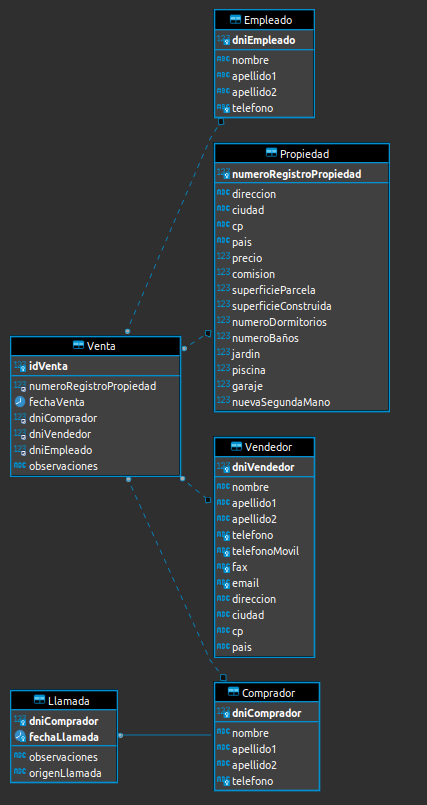
\includegraphics[scale = 0.75]{img/E-R.png}
        \caption{Modelo E-R desde Dbeaver}
      \end{figure}
  \newpage
    \section{Vista de los registros introducidos}
      \begin{figure}[h]
        \centering
        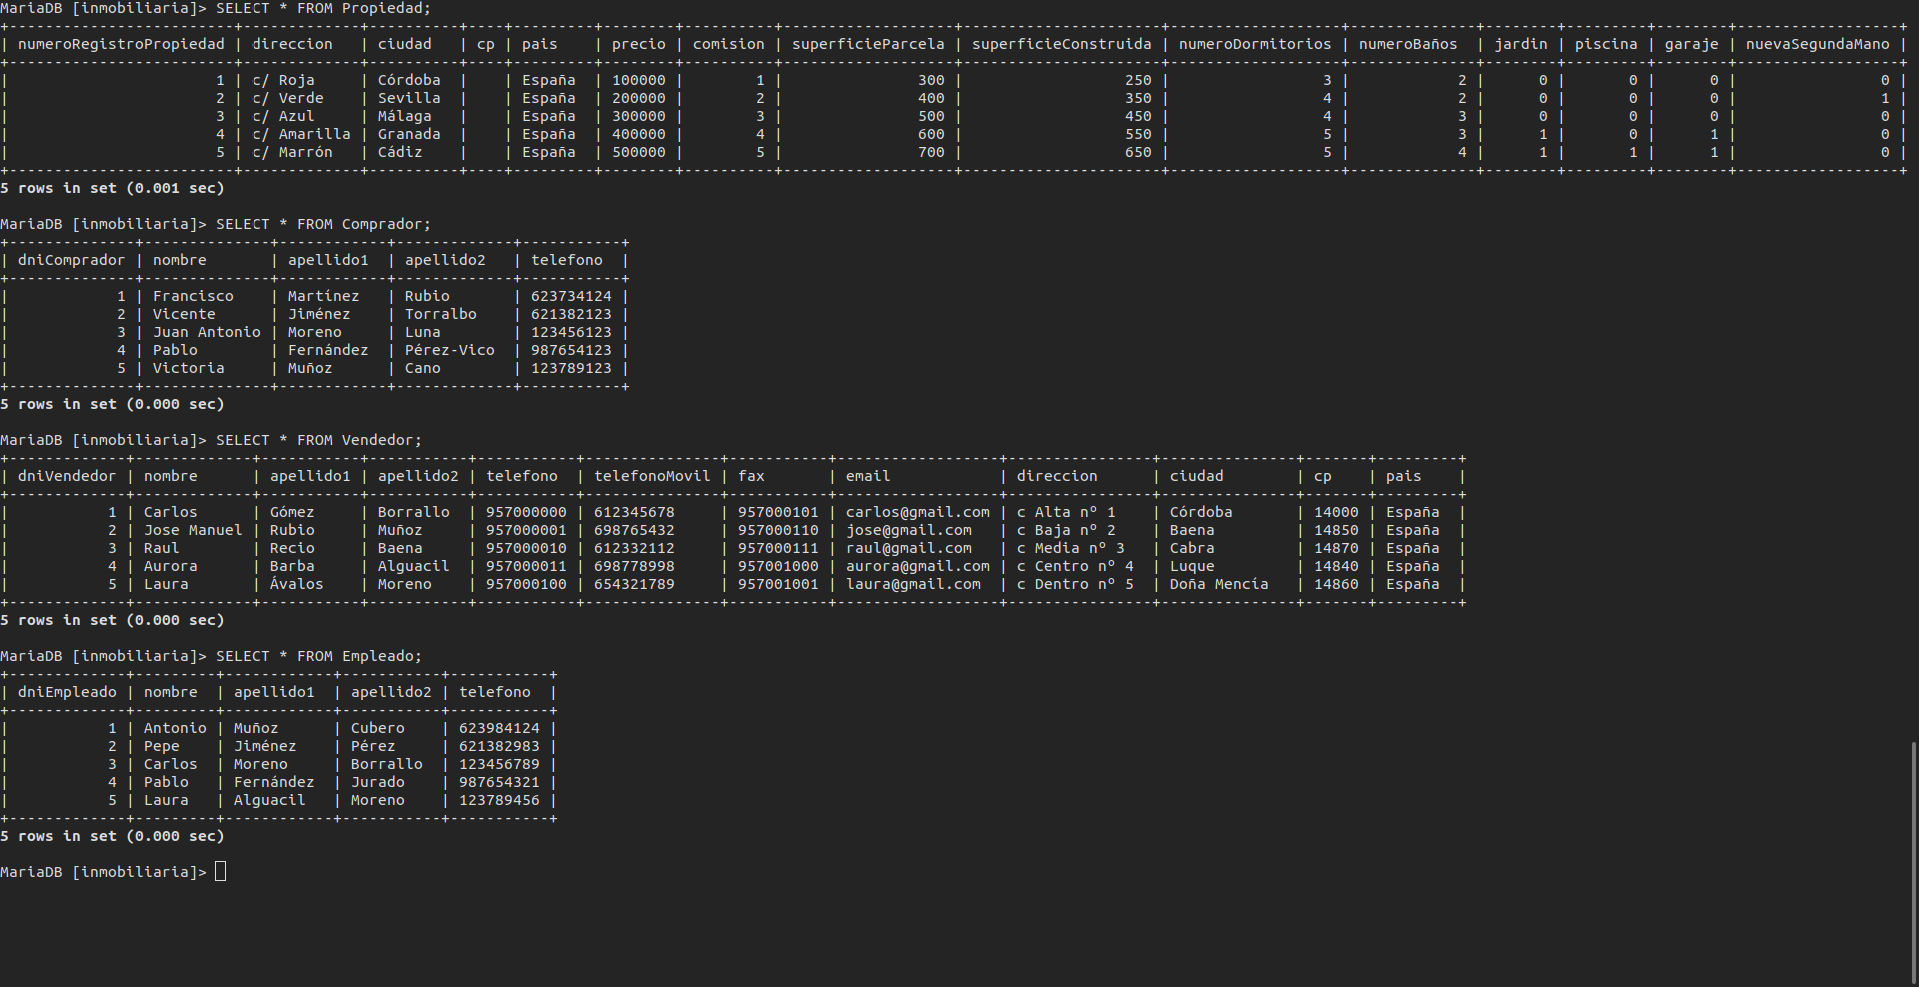
\includegraphics[scale = 0.3]{img/select.png}
        \caption{Consulta SELECT de todas las tablas.}
      \end{figure}

  \newpage
    \listoffigures

\end{document}